\chapter{Unicast Routing}
\label{chap:unicast}

This section describes the structure of unicast routing in \ns.
We begin by describing
\href{the interface to the user}{Section}{sec:API},
through methods in the \clsref{Simulator}{../ns-2/ns-lib.tcl}
and the \clsref{RouteLogic}{../ns-2/ns-lib.tcl}.
We then describe
\href{configuration mechanisms for specialized routing}{%
        Section}{sec:uni:specroute}
such as asymmetric routing, or equal cost multipath routing
The next section describes the
\href{the configuration mechanisms for individual routing strategies
and protocols}{Section}{sec:uni:protconfig}.
We conclude with a comprehensive look at 
\href{the internal architecture}{Section}{sec:rtg-internals}
of routing in \ns.

The procedures and functions described in this chapter can be found in
\nsf{tcl/lib/ns-route.tcl}, \nsf{tcl/rtglib/route-proto.tcl}, 
\nsf{tcl/mcast/McastProto.tcl}, and \nsf{rtProtoDV.\{cc, h\}}.

\section{The Interface to the Simulation Operator (The API)}
\label{sec:API}

The user level simulation script requires one command:
to specify the unicast routing strategy or protocols for the simulation.
A routing strategy is a general mechanism by which \ns\
will compute routes for the simulation.
There are four routing strategies in \ns:
Static, Session, Dynamic and Manual.
Conversely, a routing protocol is a realization of a specific algorithm.
Currently, Static and Session routing use
the
\fcnref{Dijkstra's all-pairs SPF algorithm \cite{}}{../ns-2/route.cc}{%
        RouteLogic::compute\_routes};
one type of dynamic routing strategy is currently implemented: the
\fcnref{Distributed Bellman-Ford algorithm \cite{}}{../ns-2/route-proto.tcl}{%
        Agent/rtProto/DV::compute\_routes}.
In \ns, we blur the distinction between strategy and protocol for
static and session routing, considering them simply as protocols%
\footnote{The consideration is that static and session routing
  strategies/protocols are implemented as agents derived from
  the \clsref{Agent/rtProto},
  similar to how the different dynamic routing protocols are implemented;
  hence the blurred distinctions.}.

\fcnref{\proc[]{rtproto}}{../ns-2/route-proto.tcl}{Simulator::rtproto}
is the instance procedure in the \clsref{Simulator}{../ns-2/ns-lib.tcl}
that specifies the unicast routing protocol to be used in the simulation.
It takes multiple arguments, the first of which is mandatory;
this first argument identifies the routing protocol to be used.
Subsequent arguments specify the nodes
that will run the instance of this protocol.
The default is to run the same routing protocol
on all the nodes in the topology.
As an example, the following commands illustrate the use of the
\proc[]{rtproto} command.
\begin{program}
        $ns rtproto Static            \; Enable static route strategy for the simulation;
        $ns rtproto Session           \; Enable session routing for this simulation;
        $ns rtproto DV $n1 $n2 $n3    \; Run DV agents on nodes $n1, $n2, and $n3;
        $ns rtproto LS $n1 $n2        \; Run link state routing on specified nodes;
\end{program}
If a simulation script does not specify any \proc[]{rtproto} command,
then \ns\ will run Static routing on all the nodes in the topology.

Multiple \proc[]{rtproto} lines for the same or different routing 
protocols can occur in a simulation script.
However, a simulation cannot use both
centralized routing mechanisms such as static or session routing and 
detailed dynamic routing protocols such as DV.

In dynamic routing, each node can be running more than one routing protocol.
In such situations, more than one routing protocol can have a route to the
same destination.
Therefore, each protocol affixes a preference value to each of its routes.
These values are non-negative integers in the range 0\ldots255.
The lower the value, the more preferred the route.
When multiple routing protocol agents have a route to the same destination,
the most preferred route is chosen and
installed in the node's forwarding tables.
If more than one agent has the most preferred routes,
the ones with the lowest metric is chosen.
We call the least cost route from the most preferred protocol the
``candidate'' route.
If there are multiple candidate routes from the same or different protocols,
then, currently,
one of the agent's routes is randomly chosen\footnote{
This really is undesirable, and may be fixed at some point.
The fix will probably be to favor the agents in class preference order.
A user level simulation relying on this behavior,
or getting into this situation in specific topologies is
not recommended.}.

\paragraph{Preference Assignment and Control}
Each protocol agent stores an array of route preferences, \code{rtpref_}.
There is one element per destination, indexed by the node handle.
The default preference values used by each protocol are derived from
a class variable, \code{preference_}, for that protocol.
The current defaults are:
\begin{program}
        Agent/rtProto set preference_ 200               \; global default preference;
        Agent/rtProto/Direct\footnote{Direct is a special routing strategy that is used in conjunction with Dynamic routing.  We will describe this in greater detail as part of the route architecture description.} set preference_ 100
        Agent/rtProto/DV set preference_ 120
\end{program}
A simulation script can control routing by altering the preference
for routes in one of three ways:
alter the preference 
for a specific route learned \via\ a particular protocol agent,
alter the preference for all routes learned by the agent, or
alter the class variables for the agent before the agent is created.

\paragraph{Link Cost Assignment and Control}
In the currently implemented route protocols,
the metric of a route to a destination, at a node,
is the cost to reach the destination from that node.
It is possible to change the link costs at each of the links.
The instance procedure
\fcnref{\proc[]{cost}}{../ns-2/route-proto.tcl}{Simulator::cost}
%XXX MOVE TO NS-LIB.TCL
is invoked as \code{$ns cost \tup{node1} \tup{node2} \tup{cost}},%$
and sets the cost of the link from \tup{node1} to \tup{node2}
to \tup{cost}.
\begin{program}
        $ns cost $n1 $n2 10        \; set cost of link \textbf{from} $n1 \textbf{to} $n2 to 10;
        $ns cost $n2 $n1  5        \; set cost of link in reverse direction to 5;
        [$ns link $n1 $n2] cost?   \; query cost of link from $n1 to $n2;
        [$ns link $n2 $n1] cost?   \; query cost of link in reverse direction;
\end{program}
Notice that the procedure sets the cost along one direction only.
Similarly, the procedure
\fcnref{\proc[]{cost?}}{../ns-2/route-proto.tcl}{Link::cost?}
returns the cost of traversing the specified unidirectional link.
The default cost of a link is 1.

\section{Other Configuration Mechanisms for Specialised Routing}
\label{sec:uni:specroute}

It is possible to adjust preference and cost mechanisms to get two
special types of route configurations: 
asymmetric routing, and multipath routing.

\paragraph{Asymmetric Routing}
Asymmetric routing occurs when the path from node $n_1$ to node $n_2$
is different from the path from $n_2$ to $n_1$.
The following shows a simple topology, and cost configuration
that can achieve such a result:

\hfil
\begin{minipage}{1.85in}
Nodes $n_1$ and $n_2$ use different paths to reach each other.
All other pairs of nodes use symmetric paths to reach each other.
\end{minipage}
\hfil
\begin{minipage}{1.in}
  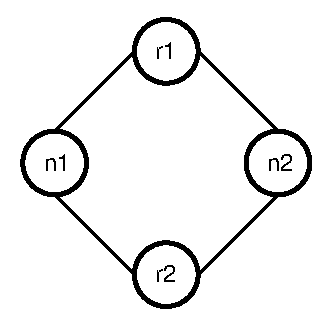
\includegraphics[height=1in]{asymmetric_routing.eps}
\end{minipage}
\hfil
\begin{minipage}{1.85in}
  \begin{program}
    $ns cost $n1 $r1 2
    $ns cost $n2 $r2 2
    $ns cost $r1 $n2 3
  \end{program}%$
\end{minipage}
\hfil

Any routing protocol that uses link costs as the metric can observe
such asymmetric routing if the link costs are appropriately configured%
\footnote{Link costs can also be used to favour or disregard
specific links in order to achieve particular topology configurations.}.

\paragraph{MultiPath Routing}
Each node can be individually configured
to use multiple separate paths to a particular destination.
The instance variable \code{multiPath_} determines whether or not
that node will use multiple paths to any destination.
Each node initialises its instance variable from a class variable
of the same name.
If multiple candidate routes to a destination are available,
all of which are learned through the same protocol,
then that node can use
all of the different routes to the destination simultaneously.
A typical configuration is as shown below:
\begin{program}
        Node set multiPath_ 1 \; All new nodes in the simulation use multiPaths where applicable;
{\rm or alternately}
        set n1 [$ns Node] \; only enable $n1 to use multiPaths where applicable;
        $n1 set multiPath_ 1
\end{program}%$
Currently, only DV routing can generate multipath routes.

\section{Protocol Specific Configuration Parameters}
\label{sec:uni:protconfig}

\paragraph{Static Routing}
The static route computation strategy is
the default route computation mechanism  in \ns.
This strategy uses the
\fcnref{Dijkstra's all-pairs SPF algorithm \cite{}}{../ns-2/route.cc}{%
        RouteLogic::compute\_routes}.
The route computation algorithm is run exactly once
prior to the start of the simulation.
The routes are computed
using an adjacency matrix and link costs of all the links in the topology.

(Note that static routing is static in the sense that it is computed
  once when the simulation starts, as opposed to session
  and DV routing that allow routes to change mid-simulation.
An alternative to static routing is Manual routing
  where routes are not computed but instead are set (manually) by the user.)

\paragraph{Session Routing}
The static routing strategy described earlier
only computes routes for the topology once in the course of a simulation.
If the above static routing is used and the topology changes while the
simulation is in progress, some sources and destinations may become
temporarily unreachable from each other for a short time.

Session routing strategy is almost identical to static routing,
in that it runs the Dijkstra all-pairs SPF algorithm
prior to the start of the simulation, using the
adjacency matrix and link costs of the links in the topology.
However, it will also run the same algorithm to recompute routes
in the event that the topology changes during the course of a
simulation. 
In other words, route recomputation and recovery is done
instantaneously and there will not be transient routing outage as in
static routing. 

Session routing provides complete and instantaneous routing changes 
in the presence of topology dynamics.
If the topology is always connected, there is
end-to-end connectivity at all times during the course of the simulation.
However, the user should note that the instantaneous route recomputation 
of session routing does not prevent temporary violations of causality,
such as packet reordering, around the instant that the topology
changes. 

\paragraph{DV Routing}
DV routing is the implementation of
Distributed Bellman-Ford (or Distance Vector) routing in \ns.
The implementation sends periodic route updates every \code{advertInterval}.
This variable is a class variable in the \clsref{Agent/rtProto/DV}{../ns-2/tcl/rtglib/route-proto.tcl}.
Its default value is 2 seconds.

In addition to periodic updates, each agent also sends triggered updates;
it does this whenever the forwarding tables in the node change.
This occurs either due to changes in the topology, 
or because an agent at the node received a route update,
and recomputed and installed new routes.

Each agent employs the split horizon with poisoned reverse mechanisms
to advertise its routes to adjacent peers.
``Split horizon'' is the mechanism by which an agent will not advertise
the route to a destination out of the interface that it is using to
reach that destination.
In a ``Split horizon with poisoned reverse'' mechanism,
the agent will advertise that route out of that interface with 
a metric of infinity.

Each DV agent uses a default \code{preference_} of 120.
The value is determined by the class variable of the same name.

Each agent uses the class variable \code{INFINITY} (set at 32)
to determine the validity of a route.


\paragraph{Manual Routing}
Manual routing is not a route computation protocol (like the others),
  but simply a way for users to configure the routing table by hand,
  much as you would with the ``route'' command on a workstation.

To use manual routing, enable it with rtproto, then set each
nodes routing tables with the add-route-to-adj-node command.
For example:
\begin{program}
$ns rtproto Manual
set n1 [$ns node]
set n2 [$ns node]
$ns duplex-link $n1 $n2 10Mb 100ms DropTail
$n1 add-route-to-adj-node -default $n2
$n2 add-route-to-adj-node -default $n1
\end{program}

For a more complete example, see \code{tcl/ex/many_tcp.tcl}.


\section{Internals and Architecture of Routing}
\label{sec:rtg-internals}

We start with a discussion of the classes associated with
unicast routing, and the code path used to configure and execute
each of the different routing protocols.
We conclude with a description of
the interface between unicast routing and network dynamics, and
that between unicast and multicast routing.

\subsection{The classes}
There are four main classes,
the class RouteLogic, the class rtObject, the class rtPeer, and the
base class Agent/rtProto for all protocols.
In addition, the routing architecture extends 
the classes Simulator, Link, Node and Classifier.

\paragraph{\protect\clsref{RouteLogic}{../ns-2/route-proto.tcl}}
This class defines two methods to configure unicast routing,
and one method to query it for route information.
It also defines an instance procedure that is applicable when
the topology is dynamic.
We discuss this last procedure in conjunction
with the interface to network dynamics.
\begin{itemize}
\item The instance procedure
\fcnref{\proc[]{register}}{../ns-2/route-proto.tcl}{RouteLogic::register}
is invoked by \proc[]{Simulator::rtproto}.
It takes the protocol and a list of nodes as arguments,
and constructs an instance variable, \code{rtprotos_}, as an array;
the array index is the name of the protocol, and the value is the list
of nodes that will run this protocol.
\item The
\fcnref{\proc[]{configure}}{../ns-2/route-proto.tcl}{RouteLogic::configure}
reads the \code{rtprotos_} instance variable, and 
for each element in the array, 
invokes route protocol methods to perform the appropriate initializations.
It is invoked by
\fcnref{the simulator run procedure}{../ns-2/ns-lib.tcl}{Simulator::run}.

For each protocol \tup{rt-proto} indexed in the \code{rtprotos_} array,
this routine invokes
\code{Agent/rtProto/\tup{rt-proto} init-all rtprotos_(\tup{rt-proto})}.

If there are no elements in \code{rtprotos_},
the routine invokes Static routing, as
\code{Agent/rtProto/Static init-all}.

\item The instance procedure
\fcnref{\proc[]{lookup}}{../ns-2/route-proto.tcl}{RouteLogic::lookup}
takes two node numbers, $nodeId_1$ and $nodeId_2$, as argument;
it returns the id of the neighbor node that $nodeId_1$ uses to 
reach $nodeId_2$.

The procedure is used by the static route computation procedure to query
the computed routes and populate the routes at each of the nodes.
It is also used by the multicast routing protocols to perform the
appropriate RPF check.

Note that this procedure overloads an instproc-like of the same name.
The procedure queries the appropriate \code{rtObject} entities
if they exist
(which they will if dynamic routing strategies are used in the simulation);
otherwise, the procedure invokes the instproc-like to obtain the relevant
information.
\end{itemize}

\paragraph{\protect\clsref{rtObject}{../ns-2/route-proto.tcl}}
is used in simulations that use dynamic routing.
Each node has a rtObject associated with it, that
acts as a co-ordinator for the different routing protocols that
operate at a node.
At any node, the rtObject at that node 
tracks each of the protocols operating at that node;
it computes and installs the nest route to each destination
available via each of the protocols.
In the event that the routing tables change, or the topology changes,
the rtObject will alert the protocols to take the appropriate action.

The class defines the procedure
\fcnref{\proc[]{init-all}}{../ns-2/route-proto.tcl}{rtObject::init-all};
this procedure takes a list of nodes as arguments,
and creates a rtObject at each of the nodes in its argument list.
It subsequently invokes its \code{compute-routes}.

The assumption is that the constructor for each of the new objects
will instantiate the ``Direct'' route protocol at each of these nodes.
This route protocol is responsible for computing the routes to 
immediately adjacent neighbors.
When \proc[]{compute-routes} is run by the \proc[]{init-all} 
procedure, these direct routes are installed in the node by the
appropriate route object.

The other instance procedures in this class are:
\begin{itemize}
\item \fcnref{\proc[]{init}}{../ns-2/route-proto.tcl}{rtObject::init}
The constructor sets up pointers from itself to the node,
in its instance variable \code{node_}, and from the node to itself,
through the Node instance procedure
\proc[]{init-routing} and the Node instance variable \code{rtObject_}.
It then initializes an array of
\code{nextHop_}, \code{rtpref_}, \code{metric_}, \code{rtVia_}.
The index of each of these arrays is the handle of the destination node.

The \code{nextHop_} contains the link that will be used to reach the
particular destination;
\code{rtpref_} and \code{metric_} are
the preference and metric for the route installed in the node;
\code{rtVia_} is the name of the agent whose route is installed in the node.

The constructor also creates the instance of the Direct route protocol,
and invokes \proc[]{compute-routes} for that protocol.

\item
\fcnref{\proc[]{add-proto}}{../ns-2/route-proto.tcl}{rtObject::add-proto}
creates an instance of the protocol, stores a reference to it
in its array of protocols, \code{rtProtos_}.
The index of the array is the name of the protocol.
It also attaches the protocol object to the node,
and returns the handle of the protocol object.

\item \fcnref{\proc[]{lookup}}{../ns-2/route-proto.tcl}{rtObject::lookup}
takes a destination node handle, and returns the id of the neighbor node
that is used to reach the destination.

If multiple paths are in use, then it returns a list of the
neighbor nodes that will be used.

If the node does not have a route to the destination,
the procedure will return -1.

\item
\fcnref{\proc[]{compute-routes}}{../ns-2/route-proto.tcl}{rtObject::compute-routes}
is the core procedure in this class.
It first checks to see if any of the routing protocols
at the node have computed any new routes.
If they have,
it will determine the best route to each destination
from among all the protocols.
If any routes have changed,
the procedure will notify each of the protocols of the number of
such changes, in case any of these protocols wants to send a fresh update.
Finally, it will also notify any multicast protocol that new unicast route
tables have been computed.

The routine checks the protocol agent's instance variable,
\code{rtsChanged_} to see if any of the routes in that protocol
have changed since the protocol was last examined.
It then uses the protocol's instance variable arrays,
\code{nextHop_}, \code{rtpref_}, and \code{metric_}
to compute its own arrays.
The rtObject will install or modify any of the routes as the changes are found.

If any of the routes at the node have changed,
the rtObject will invoke the protocol agent's instance procedures,
\proc[]{send-updates} with the number of changes as argument.
It will then invoke the multicast route object, if it exists.
\end{itemize}

The next set of routines are used to query the rtObject for various state
information.
\begin{itemize}
\item
\fcnref{\proc[]{dump-routes}}{../ns-2/route-proto.tcl}{rtObject::dump-routes}
takes a output file descriptor as argument, and writes out the
routing table at that node on that file descriptor.

A typical dump output is:
{\small
\begin{verbatim}
\end{verbatim}
}

\item
\fcnref{\proc[]{rtProto?}}{../ns-2/route-proto.tcl}{rtObject::rtProto?}
takes a route protocol as argument, and returns a handle to the instance
of the protocol running at the  node.

\item
\fcnref{\proc[]{nextHop?}}{../ns-2/route-proto.tcl}{rtObject::nextHop?}
takes a destination node handle, and returns the link that is used to reach
that destination.

\item
Similarly,
\fcnref{\proc[]{rtpref?}}{../ns-2/route-proto.tcl}{rtObject::rtpref?} and
\fcnref{\proc[]{metric?}}{../ns-2/route-proto.tcl}{rtObject::metric?}
take a destination node handle as argument, and return the preference
and metric of the route to the destination installed at the node.
\end{itemize}

\paragraph{The \protect\clsref{rtPeer}{../ns-2/route-proto.tcl}}
is a container class used by the protocol agents.
Each object stores the address of the peer agent, and the 
metric and preference for each route advertised by that peer.
A protocol agent will store one object per peer.
The class maintains the instance variable \code{addr_}, and the
instance variable arrays, \code{metric_} and \code{rtpref_};
the array indices are the destination node handles.

The class instance procedures,
\fcnref{\proc[]{metric}}{../ns-2/route-proto.tcl}{rtPeer::metric} and
\fcnref{\proc[]{preference}}{../ns-2/route-proto.tcl}{rtPeer::preference},
take one destination and value, and set the respective array variable.
The procedures,
\fcnref{\proc[]{metric?}}{../ns-2/route-proto.tcl}{rtPeer::metric?} and
\fcnref{\proc[]{preference?}}{../ns-2/route-proto.tcl}{rtPeer::preference?},
take a destination and return the current value for that destination.
The instance procedure
\fcnref{\proc[]{addr?}}{../ns-2/route-proto.tcl}{rtPeer::addr?}
returns the address of the peer agent.

\paragraph{\protect\clsref{Agent/rtProto}{../ns-2/route-proto.tcl}}
This class is the base class from
which all routing protocol agents are derived.
Each protocol agent must define the procedure\proc[]{init-all}
to initialize the complete protocol,
and possibly instance procedures \proc[]{init}, \proc[]{compute-routes}, and
\proc[]{send-updates}.
In addition, if the topology is dynamic, and the protocol supports 
route computation to react to changes in the topology,
then the protocol should define the procedure \proc[]{compute-all}, and
possibly the instance procedure \proc[]{intf-changed}.
In this section, we will briefly describe the interface for the basic
procedures.
We will defer the description of \proc[]{compute-all} and
\proc[]{intf-changed}
to the section on network dynamics.
We also defer the description of the details of each of the protocols
to their separate section at the end of the chapter.
\begin{list}{---}{}
\item
The procedure
\fcnref{\proc[]{init-all}}{../ns-2/route-proto.tcl}{Agent/rtProto::init-all}
is a global initialization procedure for the class.
It may be given a list of the nodes as an argument.
This the list of nodes that should run this routing protocol.
However, centralized routing protocols such as static and session routing
will ignore this argument;
detailed dynamic routing protocols such as DV will use this argument
list to instantiate protocols agents at each of the nodes specified.

Note that derived classes in OTcl do not inherit the procedures
defined in the base class. 
Therefore, every derived routing protocol class must define its own
procedures explicitly.

\item
The instance procedure
\fcnref{\proc[]{init}}{../ns-2/route-proto.tcl}{Agent/rtProto::init}
is the constructor for protocol agents that are created.
The base class constructor initializes the default preference 
for objects in this class,
identifies the interfaces incident on the node and their current status.
The interfaces are indexed by the neighbor handle and stored in the instance
variable array, \code{ifs_};
the corresponding status instance variable array is \code{ifstat_}.

Centralized routing protocols such as static and session routing do not
create separate agents per node, and therefore do not access any of these
instance procedures.

\item
The instance procedure
\fcnref{\proc[]{compute-routes}}{../ns-2/route-proto.tcl}{Agent/rtProto::compute-routes}
computes the actual routes for the protocol.
The computation is based on the routes learned by the protocol, and
varies from protocol to protocol.

This routine is invoked by the rtObject whenever the topology changes.
It is also invoked when the node receives an update for the protocol.

If the routine computes new routes, 
\proc[]{rtObject::compute-routes} needs to be invoked
to recompute and possibly install new routes at the node.
The actual invoking of the rtObject is done by the procedure
that invoked this routine in the first place.

\item
The instance procedure
\fcnref{\proc[]{send-updates}}{../ns-2/route-proto.tcl}{Agent/rtProto::send-updates}
is invoked by the rtObject whenever the node routing tables have changed,
and fresh updates have to be sent to all peers.
The rtObject passes as argument the number of changes that were done.
This procedure may also be invoked when there are no changes to the routes,
but the topology incident on the node changes state.
The number of changes is used to determine the list of peers to which
a route update must be sent.
\end{list}
Other procedures relate to responding to topology changes and
\href{are described later}{Section}{sec:rtglibAPI}.

\paragraph{Other Extensions to the Simulator, Node, Link, and Classifier}
\begin{list}{---}{}
\item   % class Simulator
  We have discussed the methods \proc[]{rtproto} and \proc[]{cost}
  in the class Simulator \href{earlier}{Section}{sec:API}.
  The one other method used internally is
  \fcnref{\proc[]{get-routelogic}}{../ns-2/route-proto.tcl}{Simulator::get-routelogic};
  this procedure returns the instance of routelogic in the simulation.

  The method is used by the class Simulator, and unicast and multicast routing.

\item   % class Node
   The class Node contains these additional instance procedures
   to support dynamic unicast routing:
\fcnref{\proc[]{init-routing}}{../ns-2/route-proto.tcl}{Node::init-routing},
\fcnref{\proc[]{add-routes}}{../ns-2/route-proto.tcl}{Node::add-routes},
\fcnref{\proc[]{delete-routes}}{../ns-2/route-proto.tcl}{Node::delete-routes},
and
\fcnref{\proc[]{rtObject?}}{../ns-2/route-proto.tcl}{Node::rtObject?}.

The instance procedure \proc[]{init-routing}
is invoked by the \code{rtObject} at the node.
It stores a pointer to the rtObject, in its instance variable
\code{rtObject_}, for later manipulation or retrieval.
It also checks its class variable to see if it should use multiPath routing,
and sets up an instance variable to that effect.
If multiPath routing could be used,
the instance variable array \code{routes_} stores a count of the number of
paths installed for each destination.
This is the only array in unicast routing that is indexed by the node id,
rather than the node handle.

The instance procedure \proc[]{rtObject?}
returns the rtObject handle for that node.

The instance procedure \proc[]{add-routes}
takes a node id, and a list of links.
It will add the list of links as the routes to reach the destination
identified by the node id.
The realization of multiPath routing is done by using a separate
Classifier/multiPath.
For any given destination id $d$, if this node has multiple paths to $d$,
then the main classifier points to this multipath classifier instead of 
the link to reach the destination.
Each of the multiple paths identified by the interfaces being used is
installed in the multipath classifier.
The multipath classifier will use each of the links installed in it for
succeeding packets forwarded to it.

The instance procedure \proc[]{delete-routes}
takes a node id, a list of interfaces, and a nullAgent.
It removes each of the interfaces in the list from the installed list of
interfaces.
If the entry did not previously use a multipath classifier,
then it must have had only one route, and the route entry is set to point
to the nullAgent specified.

Q:  WHY DOES IT NOT POINT TO NULLAGENT IF THE ENTRIES IN THE MPATHCLASSIFIER
GOES TO ZERO?

\item   % class Link
  The main extension to the class Link for unicast routing is
  to support the notion of link costs.
  The instance variable \code{cost_}
  contains the cost of the unidirectional link.
  The instance procedures
  \fcnref{\proc[]{cost}}{../ns-2/route-proto.tcl}{Link::cost}
  and
  \fcnref{\proc[]{cost?}}{../ns-2/route-proto.tcl}{Link::cost?}
  set and get the cost on the link.

  Note that \proc[]{cost} takes the cost as argument.
  It is preferable to use the simulator method to set the cost variable,
  similar to the simulator instance procedures to set the queue or delay
  on a link.
  
\item   % class Classifier
The \clsref{Classifier}{../ns-2/ns-lib.tcl}
contains three new procedures, two of which overloads an existing
instproc-like, and the other two provide new functionality.

The instance procedure 
\fcnref{\proc[]{install}}{../ns-2/route-proto.tcl}{Classifier::install}
overloads the existing instproc-like of the same name.
The procedure stores the entry being installed in the instance
variable array, \code{elements_}, and then invokes the instproc-like.

The instance procedure 
\fcnref{\proc[]{installNext}}{../ns-2/route-proto.tcl}{Classifier::installNext}
also overloads the existing instproc-like of the same name.
This instproc-like simply installs the entry into the next available slot.

The instance procedure 
\fcnref{\proc[]{adjacents}}{../ns-2/route-proto.tcl}{Classifier::adjacents}
returns a list of \tup{key, value} pairs of all elements installed in the
classifier.
\end{list}

\subsection{Interface to Network Dynamics and Multicast}
\label{sec:rtglibAPI}
This section describes the methods applied in unicast routing to respond
to changes in the topology.
The complete sequence of actions that cause the changes in the topology,
and fire the appropriate actions is described in a different section.
% NEED XREF
The response to topology changes falls into two categories:
actions taken by individual agents at each of the nodes, and
actions to be taken globally for the entire protocol.

Detailed routing protocols such as the DV implementation
require actions to be performed by individual protocol agents at the
affected nodes.
Centralized routing protocols such as static and session routing fall into
the latter category exclusively.
Detailed routing protocols could use such techniques to gather statistics
related to the operation of the routing protocol;
however, no such code is currently implemented in \ns.

\paragraph{Actions at the individual nodes}
Following any change in the topology,
the network dynamics models will first invoke
\fcnref{\proc[]{rtObject::intf-changed}}{../ns-2/route-proto.tcl}{rtObject:;intf-changed}
at each of the affected nodes.
For each of the unicast routing protocols operating at that node,
\proc[]{rtObject::intf-changed} will invoke 
each individual protocol's instance procedure,  \proc[]{intf-changed},
followed by that protocol's \proc[]{compute-routes}.

After each protocol has computed its individual routes
\proc[]{rtObject::intf-changed} invokes \proc[]{compute-routes}
to possibly install new routes.
If new routes were installed in the node,
\proc[]{rtObject::compute-routes} will invoke
\proc[]{send-updates} for each of the protocols operating at the node.
The procedure will also
\fcnref{flag the multicast route
        object}{../ns-2/route-proto.tcl}{rtObject::flag-multicast}
of the route changes at the node, indicating the number of changes 
that have been executed.
\proc[]{rtObject::flag-multicast} will, in turn, notify
the multicast route object to take appropriate action.

The one exception
to the interface between unicast and multicast routing is the interaction
between dynamic dense mode multicast and detailed unicast routing.
This dynamicDM implementation in \ns\ assumes neighbor nodes
will send an implicit update whenever their routes change,
without actually sending the update.  
It then uses this implicit information to compute
appropriate parent-child relationships for the multicast spanning trees.
Therefore, detailed unicast routing will invoke
\code{rtObject_ flag-multicast 1} whenever it receives a route update as well,
even if that update does not result in any change in its own routing tables.

\paragraph{Global Actions}
Once the detailed actions at each of the affected nodes is completed,
the network dynamics models will
\fcnref{notify the RouteLogic instance (\proc[]{RouteLogic::notify})}{%
        ../ns-2/route-proto.tcl}{RouteLogic::notify} 
of changes to topology.
This procedure invokes the procedure \proc[]{compute-all}
for each of the protocols that were ever installed at any of the nodes.
Centralized routing protocols such as session routing use this signal to
recompute the routes to the topology.
Finally, the \proc[]{RouteLogic::notify} procedure notifies 
any instances of centralized multicast that are operating at the node.

\section{Protocol Internals}
\label{sec:protocol-internals}

In this section, we describe any leftover details of each of the routing
protocol agents.
Note that this is the only place where we describe the
internal route protocol agent, ``Direct'' routing.

\paragraph{Direct Routing}
This protocol tracks the state of the incident links,
and maintains routes to immediately adjacent neighbors only.
As with the other protocols, it maintains instance variable arrays
of \code{nextHop_}, \code{rtpref_}, and \code{metric_}, indexed by 
the handle of each of the possible destinations in the topology.

The instance procedure
\fcnref{\proc[]{compute-routes}}{../ns-2/route-proto.tcl}{Agent/rtProto/Direct::compute-routes}
computes routes based on the current state of the link, and the previously
known state of the incident links.

No other procedures or instance procedures are defined for this protocol.

\paragraph{Static Routing}
The procedure
\fcnref{\proc[]{compute-routes}}{../ns-2/ns-lib.tcl}{RouteLogic::compute-routes}
in the \clsref{RouteLogic}{../ns-2/ns-lib.tcl}
first creates the adjacency matrix, and then
invokes the C++ method, \fcn[]{compute\_routes} of the shadow object.
Finally, the procedure retrieves the result of the route computation,
and inserts the appropriate routes at each of the nodes in the topology.

The class only defines the procedure
\fcnref{\proc[]{init-all}}{../ns-2/route-proto.tcl}{Agent/rtProto/Static::init-all}
that invokes \proc[]{compute-routes}.

\paragraph{Session Routing}
The class defines the procedure
\fcnref{\proc[]{init-all}}{../ns-2/route-proto.tcl}{Agent/rtProto/Session::init-all}
to compute the routes at the start of the simulation.
It also defines the procedure
\fcnref{\proc[]{compute-all}}{../ns-2/route-proto.tcl}{Agent/rtProto/Session::compute-all}
to compute the routes when the topology changes.
Each of these procedures directly invokes \proc[]{compute-routes}.

\paragraph{DV Routing}
In a dynamic routing strategy, nodes send and receive messages,
and compute the routes in the topology based on the messages exchanged.
The procedure
\fcnref{\proc[]{init-all}}{../ns-2/route-proto.tcl}{Agent/rtProto/DV::init-all}
takes a list of nodes as the argument;
the default is the list of nodes in the topology.
At each of the nodes in the argument, the procedure starts the
\clsref{rtObject}{../ns-2/route-proto.tcl} and a 
\clsref{Agent/rtProto/DV}{../ns-2/route-proto.tcl} agents.
It then determines the DV peers for each of the newly created DV agents,
and creates the relevant \code{rtPeer} objects.

The
\fcnref{constructor for the DV agent}{%
        ../ns-2/route-proto.tcl}{Agent/rtProto/DV::init}
initializes a number of instance variables;
each agent stores an array, indexed by the destination node handle,
of the preference and metric, the interface (or link) to the next hop,
and the remote peer incident on the interface,
for the best route to each destination computed by the agent.
The agent creates these instance variables, and then
schedules sending its first update within the first
0.5 seconds of simulation start.

Each agent stores the list of its peers indexed by the handle
of the peer node.
Each peer is a separate peer structure that holds
the address of the peer agent, the metric and preference
of the route to each destination advertised by that peer.
We discuss the rtPeer structure later
when discuss the route architecture.
The peer structures are initialized by the procedure
\fcnref{\proc[]{add-peer}}{../ns-2/route-proto.tcl}{Agent/rtProto/DV::add-peer}
invoked by \proc[]{init-all}.

The routine 
\fcnref{\proc[]{send-periodic-update}}{../ns-2/route-proto.tcl}{Agent/rtProto/DV::send-periodic-update}
invokes \proc[]{send-updates} to send the actual updates.
It then reschedules sending the next periodic update
after \code{advertInterval} jittered slightly to avoid
possible synchronization effects.

\fcnref{\proc[]{send-updates}}{../ns-2/route-proto.tcl}{Agent/rtProto/DV::send-updates}
will send updates to a select set of peers.
If any of the routes at that node have changed, or for periodic updates,
the procedure will send updates to all peers.
Otherwise, if some incident links have just recovered,
the procedure will send updates to the adjacent peers on those incident
links only.

\proc[]{send-updates} uses the procedure
\fcnref{\proc[]{send-to-peer}}{../ns-2/route-proto.tcl}{Agent/rtProto/DV::send-to-peer}
to send the actual updates.
This procedure packages the update, taking the
split-horizon and poison reverse mechanisms into account.
It invokes the instproc-like,
\fcnref{\proc[]{send-update} (Note the singular case)}{%
        ../ns-2/rtProto.cc}{rtProtoDV::command}
to send the actual update.
The actual route update is stored in the class variable
\code{msg_} indexed by a non-decreasing integer as index.
The instproc-like only sends the index to \code{msg_} to the remote peer.
This eliminates the need to convert from OTcl strings to alternate formats
and back.

When 
\fcnref{a peer receives a route update}{../ns-2/route-proto.tcl}{%
        Agent/rtProto/DV::recv-update}
it first checks to determine if the update from differs from the previous
ones.
The agent will compute new routes if the update contains new information.


\section{Unicast routing objects}
\label{sec:routeobjects}

Routelogic and rtObject are two objects that are significant to unicast
routing in \ns. Routelogic, essentially, represents the routing table
that is created and maintained centrally for every unicast simulation.
rtObject is the object that every node taking part in dynamic
unicast routing, has an instance of. Note that nodes will not have an
instance of this object if Session routing is done as a detailed
routing protocol is not being simulated in this case. The methods for
RouteLogic and rtObject are described in the next section.


\section{Commands at a glance}
\label{sec:unicastcommand}

Following is a list of unicast routing related commands used in simulation
scripts:
\begin{flushleft}
\code{$ns_ rtproto <routing-proto> <args>}%$

where <routing-proto> defines the type of routing protocol to be used, like
Static, Manual, Session , DV etc. args may define the list of nodes on
which the protocol is to be run. The node list defaults to all nodes in
the topology.

Internal methods:

\code{$ns_ compute-routes}%$

This command computes \code{next_hop} information for all nodes in the
topology using the topology connectivity. This \code{next_hop} info is
then used to populate the node classifiers or the routing tables.
compute-routes calls compute-flat-routes or compute-hier-routes depending
on the type of addressing being used for the simulation.

\code{$ns_ get-routelogic}%$

This returns a handle to the RouteLogic object (the routing table),
if one has been created. Otherwise a new routing table object is created.

\code{$ns_ dump-routelogic-nh}%$

This dumps next hop information in the routing table.

\code{$ns_ dump-routelogic-distance}%$

This dumps the distance information in the routing table.

\code{$node add-route <dst> <Target>}%$

This is a method used to add routing entries (nexthop information) in
the node's 
routing table. The nexthop to <dst> from this node is the <target> object
and this info is added to the node's classifier.

\code{$routelogic lookup <srcid> <destid>}%$

Returns the id of the node that is the next hop from the node with id
srcid to the node with id destid. 

\code{$routelogic dump <nodeid>}%$

Dump the routing tables of all nodes whose id is less than nodeid. Node
ids are typically assigned to nodes in ascending fashion starting from 0
by their order of creation. 

\code{rtobject dump-routes <fileID>}

Dump the routing table to the output channel specified by fileID. fileID
must be a file handle returned by the Tcl open command and it must have
been opened for writing. 

\code{$rtobject rtProto? <proto>}%$

Returns a handle to the routing protocol agent specified by proto if it
exists at that node. Returns an empty string otherwise. 

\code{$rtobject nextHop? <destID>}%$

Returns the id of the node that is the next hop to the destination
specified by the node id, <destID>. 

\code{$rtobject rtpref? destID }%$

Returns the preference for the route to destination node given by destid.

\code{$rtobject metric? destID }%$

Returns metric for the route to destid.

\end{flushleft}

\endinput

### Local Variables:
### mode: latex
### comment-column: 60
### backup-by-copying-when-linked: t
### file-precious-flag: nil
### End:
% LocalWords:  Unicast unicast API ns lib tcl RouteLogic uni specroute rtg SPF
% LocalWords:  multipath protconfig rtglib mcast McastProto rtProtoDV cc outes
% LocalWords:  rtProto DV rtproto LS rtpref eps multiPath advertInterval rtPeer
% LocalWords:  multicast rtObject rtprotos rt init RPF instproc co nextHop addr
% LocalWords:  rtVia rtProtos rtsChanged intf OTcl ifs ifstat rtglibAPI msg nh
% LocalWords:  routelogic nullAgent MPATHCLASSIFIER installNext adjacents recv
% LocalWords:  dynamicDM rtobject hier dst nexthop nodeid ids fileID destID
% LocalWords:  destid flushleft
